%%%%%%
%
% $Author: Sudhanshu Pukale $
% $Date: 18/02/2025 $
% $Pfad: manual/Contents/en/Functions.tex $
% $Version: 1 $
%
%%%%%%


\chapter{Main function}

% Main Function description and introduction

Welcome to Magic Wand with Pico4ML-BLE !.The Magic Wand project using Pico4ML-BLE is a gesture recognition system that utilizes machine learning to detect and classify hand movements \cite{arducam}. Its main function is to recognize predefined gestures, allowing users to control devices or perform actions through simple wand-like motions.

\bigskip

\textbf{The Pico4ML-BLE offers exciting key features for creating a magic wand project:}

\begin{itemize}
    \item Gesture Recognition – Detects hand-drawn shapes like Circles, Slope, and Wings.
    \item Bluetooth Connectivity: Incorporates a BLE 5.0 module for wireless communication.
    \item Google Colab Integration: Supports custom Magic Wand model training.
    \item Sensor Data Collection: Enables data acquisition via senor for collecting and training the data.
\end{itemize}



\chapter{List of Items}\label{chap:list_of_items}

\section{Inside Your Box}

Your Pico4ML-BLE kit contains:

\begin{itemize}
    \item Pico4ML-BLE Board
    \item Micro USB Cable
    \item Quick Start Guide
\end{itemize}


\begin{center}
    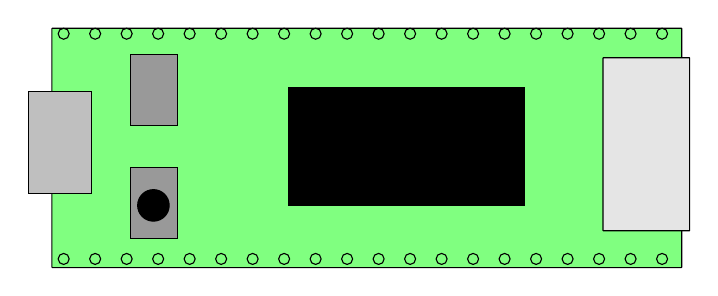
\begin{tikzpicture}[rotate=90] % Rotates the diagram horizontally
        
        % Dimensions (adjust as needed)
        \def\width{3}
        \def\height{8}
        \def\holeRadius{0.07}
        \fill[green!50] (-0.04,0) rectangle (\width,\height);
        % Board Outline
        \draw[rounded corners=0.2] (-0.04,0) rectangle (\width,\height);
        
        % Holes (Side Mounting Holes)
        \foreach \y in {0.25, 0.65, ..., \height} {
            \draw (\holeRadius,\y) circle (\holeRadius);
            \draw (\width-\holeRadius,\y) circle (\holeRadius);
        }
        
        % MICRO USB (Top Section)
        \coordinate (center) at (0.0,0.0);
        \draw[fill=gray!50] (center) ++(0.9,7.5) rectangle ++(1.3,0.8);
        
        % BOOSTEL (Component)
        \coordinate (center) at (0.5,0.5);
        \draw[fill=gray!80] (center) ++(-0.17,5.9) rectangle ++(0.9,0.6);
        
        % Small Circular Components
        \draw[fill=black] (\width/4, \height-1.29) circle (0.2);
        \draw[fill=black] (\width/1.34, \height-1.29) circle (0.2);
        
        % RUN Button (Component)
        \coordinate (center) at (0.5,0.5);
        \draw[fill=gray!80] (center) ++(1.27,5.9) rectangle ++(0.9,0.6);
        
        % LCD Display (Middle Section)
        \draw[fill=black] (\width/4, \height-3) rectangle (\width*3/4, \height-6);
        
        % Bluetooth Module (Bottom Section)
        \draw[fill=gray!20, rounded corners=0.1] (\width/7,1.0) rectangle (\width*3.5/4, -0.1);
        
    \end{tikzpicture}
    
    \captionof{figure}{Pico4ML Board}
\end{center}	


\begin{center}
    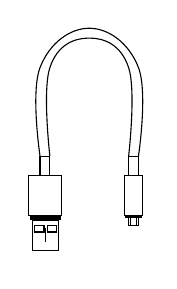
\begin{tikzpicture}[scale=0.25]
        
        \draw  (-1.5,-0.5) node (v3) {} rectangle (-1,-1.5);
        \draw  (-2.1,-1.5) rectangle (-0.4,-3.5);
        \filldraw (-2,-3.5) rectangle (-0.45,-3.7);
        \draw  (-1.9,-3.75) rectangle (-0.55,-5.3);
        \node (v2) at (-1.2,-3.65) {};
        \node (v1) at (-1.2,-5.35) {};
        \draw  (v1) edge (v2);
        \draw  (-1.8,-4) rectangle (-1.3,-4.35);
        \draw  (-1.1,-4) rectangle (-0.65,-4.35);
        \draw  plot[smooth, tension=.7] coordinates {(v3) (-1.5,4) (1,6) (3.5,4) (3.5,-0.5)};
        \draw  (3,-0.5) node (v4) {} rectangle (3.5,-1.5);
        \draw  plot[smooth, tension=.7] coordinates {(-1,-0.5) (-1,4) (1,5.5) (3,4) (v4)};
        \draw  (2.8,-1.5) rectangle (3.7,-3.5);
        \filldraw  (2.85,-3.5) rectangle (3.65,-3.6);
        \draw  (3,-3.5) rectangle (3.5,-4);
        \draw (3.1,-4) -- (3.1,-3.5);
        \draw (3.4,-4) -- (3.4,-3.5);
    \end{tikzpicture}
    \captionof{figure}{Micro USB Cable}
\end{center}



\chapter{Getting Started}\label{chap:list_of_items}

This is an application of the magic wand used to recognize gestures through an accelerometer.

\section{Unboxing the Pico4ml-BLE board}

Inside the box, you will find the Pico4ml-BLE board. Please handle it with care to avoid any breakage or serious damages.

\subsection{Check for List of Items}

The box should contain the following list of items:

\begin{itemize}
    \item Pico4ml-BLE board
    \item USB Cable
\end{itemize}

\section{Installation}
\begin{itemize}
    \item Download the magic\_wand.uf2 file from the Arducam website \URL{https://github.com/Arducam/Pico4ML-Magic-Wand/raw/main/bin/magic_wand.uf2}.
    \item Connect the Pico4ML-BLE to your computer via micro-USB while holding the BOOTSEL button.
    \item Drag and drop the file \FILE{magic\_wand.uf2}  into the RPI-RP2 window that appears.\cite{arducamBuildMagic}
\end{itemize}



\section{First Steps}

\begin{itemize}
    \item Connect to the Pico4ML-BLE via Bluetooth. Look for a device named ATB1103 MIDI XXXX1.
    
    \item Once connected, the Bluetooth button should turn green.
    
    \item Collect custom gesture data using the web interface provided by Arducam.
    
    \item Use Google Colab to train a machine learning model with your collected data.
    \item Once done, convert the header file to tflite file.
    \item Finally deploy the model in Pico4ML-BLE
\end{itemize}


\chapter{Functions}

\section{Power Supply}
% Description of product functions and keyword recognition
Connect the Cable Micro USB here for power inlet, The Power LED indicates whether the main power is connected. The light will turn to green once you connect.

\section{Capturing Movements}
Specially, the MagicWand is fitted with an advanced motion sensor for sensing practically all kinds of movements like a W (wing), O (ring), or L (slope) shape \cite{manualsArduCamB0330}. Each gesture corresponds to its own magical command.


\section{Wings}
Straighten out your arm in front of you with the wand pointed up at the top. Then drop the wand down toward your lower right; when the wand reaches an angle around halfway, lift it up toward the upper center, creating the first “V” shape. After that, drop the wand toward your lower left and then bring it up to the upper right again, completing the second “V” shape. The movements together are of a "W"-like pattern in the air. The direction of each of these movements is shown in the figure below. The wing gesture is recognized with the red color.
\begin{figure}[H]
	\centering
	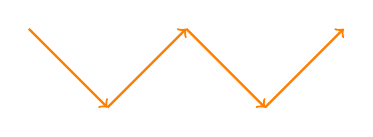
\begin{tikzpicture}
		\draw[orange, thick, ->] (0,0) -- (1,-1);
		\draw[orange, thick, ->] (1,-1) -- (2,0);
		\draw[orange, thick, ->] (2,0) -- (3,-1);
		\draw[orange, thick, ->] (3,-1) -- (4,0);
	\end{tikzpicture}
	\caption{Wing Gesture}
\end{figure}

\section{Rings}

The wand should be held upright at the center position in front of you. Move the wand in a smooth circular motion to create a ring in the air. Your circular motion should be smooth and steady, completing the circle. RIng Gesture detected-a green color is, therefore, produced.

\begin{figure}[h!]
\centering
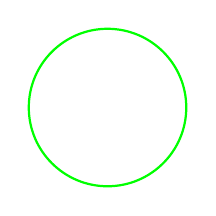
\begin{tikzpicture}
	\draw[green, thick, <-] (0,0) circle (1cm);
\end{tikzpicture}
\caption{Ring Gesture}
\end{figure}


\section{Slope}

Hold the wand by pointing it up, with the arm extended straight outside. A downward slope from the upper right to the lower left should be started. Then, move from there horizontally to the left, creating an imaginary diagonal line in the air. The blue color will be produced for slope gestures. 


\begin{figure}[h!]
	\centering
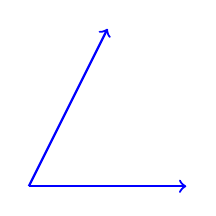
\begin{tikzpicture}
	\draw[blue, thick, ->] (0,0) -- (2,0);
	\draw[blue, thick, ->] (0,0) -- (1,2);
\end{tikzpicture}
\caption{Slope Gesture}
\end{figure}

\section{Invalid gesture}

All gestures other than mentioned previously will show on the monitor output as a cross shape.
\begin{figure}[h!]
\centering

\begin{tikzpicture}
	\draw[red, thick] (0,0) -- (2,2);
	\draw[red, thick] (2,0) -- (0,2);
\end{tikzpicture}
\caption{Invalid Gesture}
\end{figure}

\section{Reset}

\begin{itemize}
	\item Press the reset button once on the board.
	
	\item You will see all the LED lights fade out simultaneously.
	
	\item The Power LED will fade back in after clicking.
\end{itemize}

\chapter{Power OFF}
% Guide for safely powering off the Arduino Nano

To disconnect the paired Arduino Nano 33 BLE Sense from your phone and safely
power off the board, follow these steps:

\begin{itemize}
    \item \textbf{Disconnect the Bluetooth connection via your phone's settings}:
    Open the
    Bluetooth settings on your phone. Look for the Arduino Nano 33 BLE Sense in
    the list of paired or connected devices. Select the Arduino device and choose
    the option to disconnect or unpair, depending on your phone’s interface (this
    might be labeled "Unpair," "Forget," or "Disconnect")
    \item \textbf{Simply unplug the USB cable to power off the board}:
    Unlike phones or computers,
    the Arduino Nano 33 BLE Sense does not have a "power off" button or feature.
    It powers off when it is no longer receiving power. Simply disconnect the USB
    cable from the Arduino board or the power source
\end{itemize}
